%Esto es un comentario :D 
%------------------Encabezado: tiene los paquetes----------------------------------
%Empezamos definiendo que tipo de documento vamos a usar.
%respetar la gerarquía entre corchetes y llaves. Paquetes y especifidad.

\documentclass[onecolumn]{article} %report, book %números de columnos
\usepackage[spanish]{babel} %Para las cosas en español (referencias, etc) Babel puede tener problemas.
%Renombrar los comandos.
\usepackage[latin1,utf8]{inputenc} %idioma, latin1:español, inputenc es el paquete de idiomas de occidente %utf8, guión, comas, mayor que, etc, lo que se puede teclar.
\usepackage{graphics,graphicx,xcolor} %xcolor, para colores %figuras
\usepackage{amssymb,amsmath} %Lenguaje matemático %amsmath, el de las integrales
\usepackage{verbatim} %Escribir código
\usepackage{bm} %negrita

%Fecha en español. Nota: \renewcommand. También paquete para email.

%---------------------------------------------------------------------
\title{Respuestas ejercicios propuestos para Gnuplot}
\author{CARLOS ANDRES RODALLEGA MILLAN}
\date{\today}
%++++++++++++++++++++++CUERPO DEL DOCUMENTO+++++++++++++++++++++++++++
\begin{document}
\maketitle 
%.-.-.-.-.
\section{Primer punto} 
Grafica.
\begin{figure}[h!]%[h! here, para la gráfica]
	\centering %para centrar
	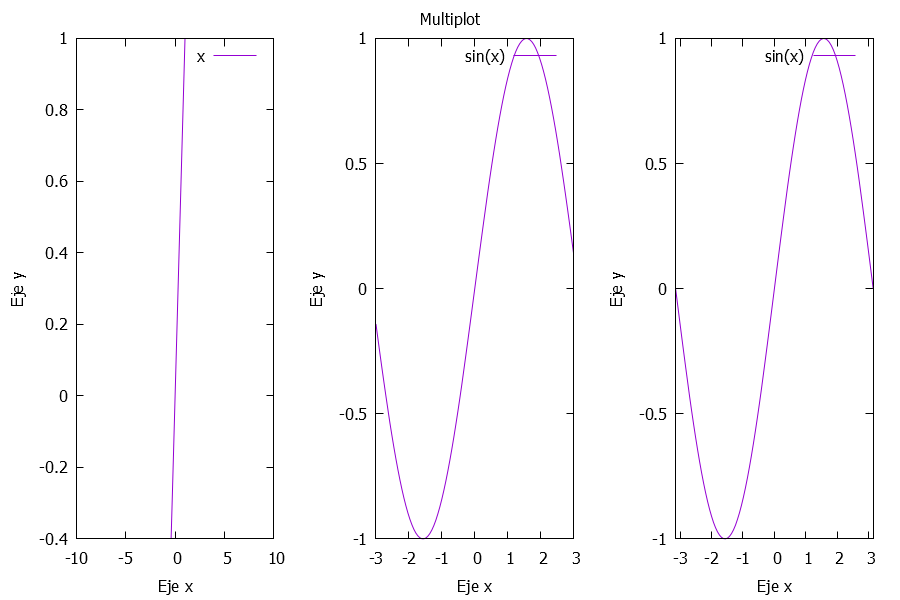
\includegraphics[scale=0.4]{Grafica_Tarea1_1.png}
	\caption{\label{fig_exp}Es una gráfica que contiene dos curvas de funciones Gaussianas, una con líneas y puntos y 		la otra con solo línea} %Enumera la gráfica.
	%Tarea, como cambiar a español.
\end{figure}
\section{Segundo Punto} 
Grafica del segundo punto.


\section{Tercer Punto}
Grafica.
\begin{figure}[h!]%[h! here, para la gráfica]
	\centering %para centrar
	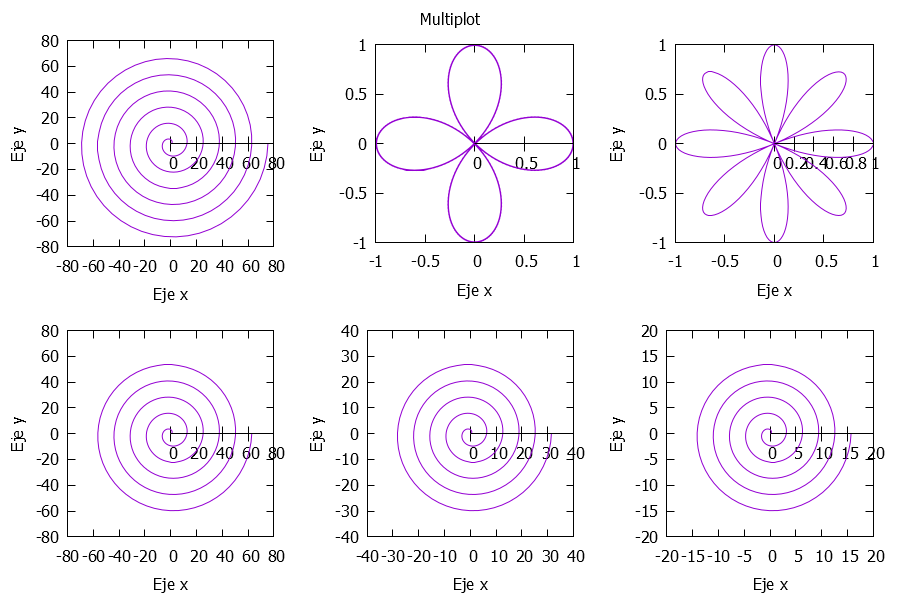
\includegraphics[scale=0.4]{grafica3.png}
	\caption{\label{fig_exp}Es una gráfica que contiene dos curvas de funciones Gaussianas, una con líneas y puntos y 		la otra con solo línea} %Enumera la gráfica.
	%Tarea, como cambiar a español.
\end{figure}
\section{Cuarto Punto}
Reproduzca el documento a continuación.

\end{document}
